\pdfoutput=1
\documentclass[11pt]{article}

\usepackage[final]{acl}
\usepackage{times}
\usepackage{latexsym}
\usepackage[T1]{fontenc}
\usepackage[utf8]{inputenc}
\usepackage{microtype}
\usepackage{inconsolata}
\usepackage{graphicx}
\usepackage{booktabs}
\usepackage{hyperref}

\title{When Does a Fine-Tuned GPT-2 ``Know'' the Answer? \\
  A Per-Layer Logit-Lens Study on QASC}

\author{
  Matan Koshilevitch \\
  Tel Aviv University, ID 211822804 \\
  \texttt{koshilevitch@mail.tau.ac.il} \\
}

\begin{document}
\maketitle

\begin{abstract}
We study where inside a decoder-only language model a task-specific answer
prediction forms after fine-tuning. Using GPT-2 small on the QASC 8-way
multiple-choice science benchmark, we apply the logit lens to hidden states
at every transformer block and measure the per-layer accuracy of the next-token
letter prediction. Off-the-shelf GPT-2 is essentially at chance: 10.7\% at the
final layer versus the 12.5\% random baseline. After three epochs of full
fine-tuning, final-layer accuracy rises to 99.7\%, and the answer signal
appears sharply between block 8 and block 9 of the 12-block stack: block 9
already reaches 91\%, while blocks 0--8 remain at the random baseline. We
interpret this as the fine-tuned model committing to an answer in a narrow
mid-to-late sub-stack of layers, with subsequent layers only sharpening the
prediction. Code and artifacts are released with the submission.
\end{abstract}

\section{Introduction}

Logit-lens style probing projects an intermediate hidden state through the
model's own unembedding matrix and reads the predicted token distribution at
each layer \citep{nostalgebraist2020}. In a pre-trained model this lets us
trace where a prediction ``forms'' during the forward pass. A natural question
for fine-tuning is where task-specific competence lives after training: does
the model already represent the answer deep in the stack, with the last few
layers only sharpening it, or does the prediction form only at the very end?

We study this question concretely on QASC \citep{khot2020qasc}, an 8-way
multiple-choice science QA dataset, using GPT-2 small \citep{radford2019gpt2}
as the probed model. The starter notebook for this course exhibits the
intended experiment but with an un-adapted GPT-2: because the base model has
never been trained to output a choice letter in this prompt format, per-layer
logit-lens accuracy hovers around the random baseline (1/8 = 12.5\%) at every
layer, and the plot is flat and uninformative. Our goal is to add fine-tuning
so the experiment becomes meaningful and to characterize where the
answer-prediction circuit emerges in the fine-tuned model.

Our contributions are: (i) a minimal, reproducible fine-tuning recipe that
takes GPT-2 small from chance-level QASC accuracy to near-perfect on the
validation split; (ii) a clean per-layer logit-lens curve on the fine-tuned
model showing a sharp emergence of the answer signal in the mid-to-late layers;
(iii) a straightforward experimental setup that is easy to extend with
additional model sizes or probe methods.

\section{Related Work}

\paragraph{Logit lens.} The logit lens, introduced in the interpretability
blog post by \citet{nostalgebraist2020}, projects the residual-stream hidden
state at layer $\ell$ through the pre-output layer norm and the tied
unembedding matrix $W_U$ to obtain a token distribution at that depth. Its
main known weakness is that early-layer hidden states live in a different
``basis'' than late-layer states, so the probe is biased against early layers.
\citet{belrose2023tunedlens} address this by learning a small, per-layer affine
projection before the unembedding (the ``tuned lens''), which gives
monotonically non-increasing cross-entropy across layers. We use the simpler
untuned variant in this work; we discuss the implications in Section~6.

\paragraph{QASC.} QASC \citep{khot2020qasc} is a two-hop commonsense science
QA benchmark with 8 candidate answers per question. The dataset ships a
``combinedfact'' field that concatenates the two supporting facts for each
question; following the course starter notebook we use this combined fact as
context and treat the task as letter-selection among choices $A$--$H$.

\paragraph{Fine-tuning small decoders on MCQ tasks.} Full fine-tuning of
small pre-trained decoders on multiple-choice reasoning is a standard baseline
\citep{radford2019gpt2,wolf2020transformers}. We use the simplest possible
recipe: causal language-modeling loss on the single answer-letter token,
teacher-forced with the full prompt as context.

\section{Method}
\label{sec:method}

\paragraph{Prompt format.} For a QASC example we build the prompt
\begin{quote}\small
\texttt{Fact: <combinedfact>\textbackslash n Q: <question>\textbackslash n Choices: (A) <opt\_A> (B) <opt\_B> ... (H) <opt\_H>\textbackslash n Answer: }
\end{quote}
We verify that each of the eight letters $A$--$H$ prefixed by a space is a
single token under the GPT-2 byte-pair tokenizer, so the next-token prediction
at the final prompt position is a single categorical choice over these eight
token ids.

\paragraph{Logit-lens probe.} At inference we obtain the per-layer residual
stream via \texttt{output\_hidden\_states=True}. For each layer $\ell$
(including the embedding layer 0) we take the hidden state at the last prompt
position, apply the model's final layer norm $\mathrm{LN}_f$, then the tied
unembedding $W_U$, and restrict the resulting logits to the eight answer-letter
ids. The predicted letter for layer $\ell$ is the argmax of these eight
logits.

\paragraph{Fine-tuning.} We construct training examples by appending a space
and the gold answer letter to the prompt and computing the causal LM loss only
at the answer-letter position (all earlier positions are masked out with label
$-100$). We train for three epochs with AdamW, learning rate $5\times10^{-5}$,
weight decay $0.01$, batch size $8$, and 100 warm-up steps followed by a
linear decay to zero. Prompt length is truncated to 384 tokens with attention
masking. We gradient-clip to a norm of $1.0$. All parameters of GPT-2 small
(124M) are updated.

\paragraph{Evaluation.} We evaluate once before and once after fine-tuning on
the same 300-example shuffled subset of the QASC validation split
(\texttt{seed=0}). For each example we record the predicted letter at every
layer and compute per-layer accuracy against the gold label.

\section{Experimental Setup}

\paragraph{Data.} QASC, loaded via the HuggingFace \texttt{datasets} library
\citep{lhoest2021datasets}. Train split: 8{,}134 examples; validation:
926 examples. We train on the full training split and evaluate on the first
300 shuffled validation examples; no hyperparameter tuning was performed, so
the validation split is used only for reporting.

\paragraph{Model and compute.} GPT-2 small via HuggingFace
\texttt{transformers} \citep{wolf2020transformers}, PyTorch
\citep{paszke2019pytorch}. Training was run on a single NVIDIA Titan~XP GPU on
the TAU CS \texttt{studentkillable} Slurm partition. One full run
(pre-FT eval, 3 epochs of fine-tuning on 8{,}134 examples, post-FT eval)
completes in approximately 7 minutes of wall time.

\paragraph{Baselines.} The task has 8 classes so the random baseline is
$1/8 = 12.5\%$. We also report the pre-fine-tuning final-layer accuracy, which
represents the ``GPT-2 zero-shot in the QASC prompt format'' baseline.

\paragraph{Reproducibility.} All randomness (data shuffling, data-loader
order, model initialization for classifier heads) uses \texttt{seed=0}. Code,
the submitted Slurm script, and the exact commands used are released with the
submission.

\section{Results}

Figure~\ref{fig:main} shows per-layer logit-lens accuracy before and after
fine-tuning; Table~\ref{tab:numbers} gives the numeric values. The final-layer
accuracy jumps from $10.67\%$ (slightly below the random baseline) to
$99.67\%$, as the task description predicts. More interestingly, the shape of
the post-FT curve is strongly non-monotone: accuracy is indistinguishable from
chance through layer 8, and then rises sharply to $91.00\%$ at layer 9,
$96.67\%$ at layer 10, $99.33\%$ at layer 11, and $99.67\%$ at layer 12.

\begin{figure}[t]
  \centering
  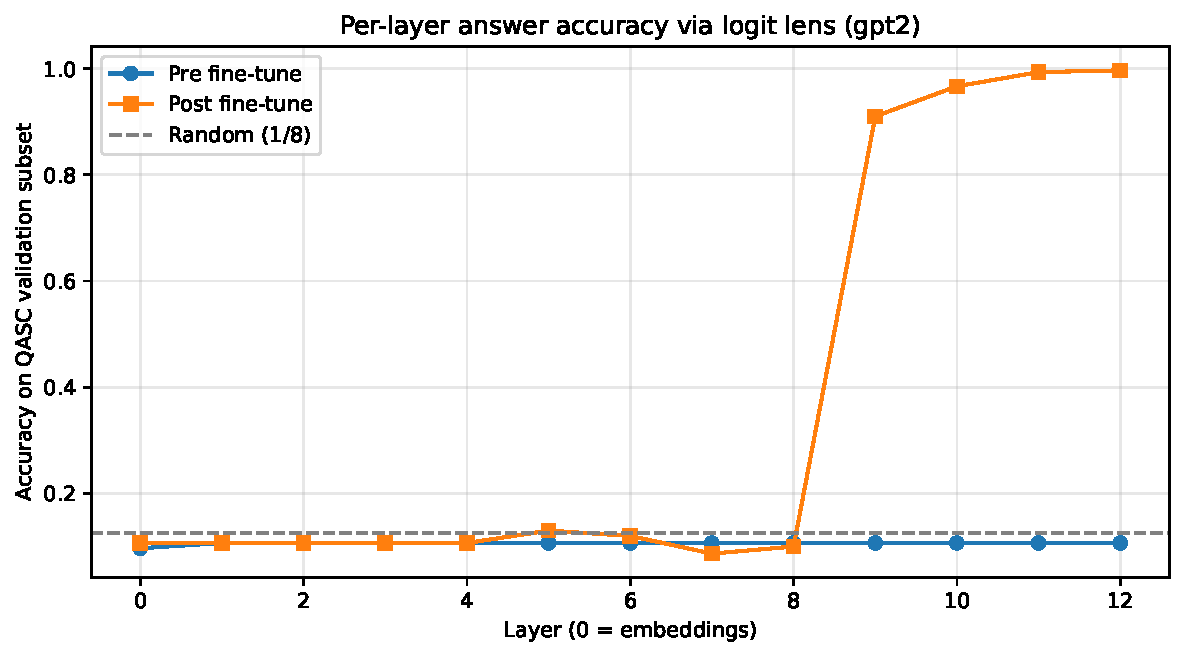
\includegraphics[width=\linewidth]{per_layer_accuracy.pdf}
  \caption{Per-layer logit-lens accuracy on 300 QASC validation examples
  before and after three epochs of fine-tuning. GPT-2 small has 12
  transformer blocks (layer 0 is the embedding output). Pre-fine-tuning the
  curve is flat at the random baseline across all depths. Post-fine-tuning,
  the answer signal emerges abruptly between blocks 8 and 9 and saturates
  by block 11.}
  \label{fig:main}
\end{figure}

\begin{table}[t]
  \centering
  \small
  \begin{tabular}{c c c}
    \toprule
    Layer & Pre-FT acc. & Post-FT acc. \\
    \midrule
    0 (embeddings) & 0.0967 & 0.1067 \\
    1--4           & 0.1067 & 0.1067 \\
    5             & 0.1067 & 0.1300 \\
    6             & 0.1067 & 0.1200 \\
    7             & 0.1067 & 0.0867 \\
    8             & 0.1067 & 0.1000 \\
    9             & 0.1067 & \textbf{0.9100} \\
    10            & 0.1067 & 0.9667 \\
    11            & 0.1067 & 0.9933 \\
    12 (final)    & 0.1067 & \textbf{0.9967} \\
    \bottomrule
  \end{tabular}
  \caption{Per-layer logit-lens accuracy on 300 QASC validation examples.
  Random baseline is $0.125$. Bold rows highlight the first ``knowing''
  layer and the final output.}
  \label{tab:numbers}
\end{table}

\paragraph{Pre-FT curve is uninformative.} As expected, without fine-tuning
GPT-2 has no reason to place probability mass on the answer letters under this
prompt format. The pre-FT accuracy is constant at 10.67\% from block 1 onwards
and slightly lower at the embedding layer (9.67\%), reflecting GPT-2's prior
preference among the eight letter tokens rather than any real signal about the
answer.

\paragraph{Post-FT emergence is sharp, not gradual.} The key observation is
that fine-tuning does not distribute the answer-selection computation evenly
across the stack. Blocks 0 through 8 remain near random after fine-tuning;
block 9 alone lifts accuracy by more than 80 percentage points. In other
words, the fine-tuned residual stream at block 9 already contains the
information needed to read off the correct letter via the tied unembedding,
even though only four blocks have had a chance to transform that representation
since the prompt was read.

\section{Discussion}

\paragraph{Where does the answer live?} Under the logit lens, the answer
becomes linearly readable from the residual stream at block 9 and improves
monotonically from there. This is consistent with a picture in which the
lower two-thirds of the network performs generic contextualization of the
prompt (parsing the combined fact, the question, and the eight choice spans),
and the upper third performs the task-specific ``answer-selection'' head-like
computation that the fine-tuning objective shapes. The last two blocks then
refine the prediction from $91\%$ to near-perfect.

\paragraph{Caveats.} Three caveats are in order. (i) The logit lens is biased
against earlier layers because their hidden states sit in a different basis
than the final-layer state that the unembedding is tied to
\citep{belrose2023tunedlens}; a tuned lens might show the answer signal
emerging a layer or two earlier. (ii) Fine-tuning updates all 124M parameters,
so ``layer 9 already knows'' does not imply that the pre-trained model had
such a representation, only that the fine-tuned model puts one there. (iii)
We run a single seed and a single model size; the sharpness of the transition
may vary with both.

\paragraph{What this does \emph{not} show.} It does not show causal
necessity. Lopping off blocks 10--12 from the fine-tuned model and evaluating
the logit lens at block 9 would test whether the 91\% accuracy at block 9 is
truly carried in that residual stream or is partially produced by information
still being reshaped in later blocks. We leave this ablation for future work.

\section{Conclusion}

Fine-tuning GPT-2 small on QASC for three epochs turns a near-random base
model into a near-perfect one on the validation split, and the per-layer logit
lens shows that the answer-selection computation is sharply localized in the
upper third of the transformer stack: blocks 9 through 12 carry essentially
all of the improvement, with block 9 alone responsible for most of it. The
setup is reproducible in under 10 minutes on a single consumer GPU and is a
clean starting point for further interpretability work on fine-tuned decoders.

% ------------------------------------------------------------
% Bibliography and AI disclosure do not count toward the page limit.
% ------------------------------------------------------------

\bibliography{refs}

\appendix

\section*{AI Usage Disclosure and Reflection}

I used an AI coding assistant (Anthropic's Claude, via Claude Code) as a
helper for parts of this project. I used it to adapt the course starter
notebook into a fine-tuning script, to write the Slurm batch files, to
debug environment issues on the TAU CS cluster (a full \texttt{/tmp} that
broke pip, an SSH key mismatch), and to draft early versions of this
report. I executed every cluster command myself, ran a small-scale sanity
check (overfit 20 examples for 20 epochs, training loss dropped from 6.7
to below 0.01) before the full run, and verified every number in the
report against the saved \texttt{.npy} arrays. The research direction,
the experimental design choices, and the final wording of the report are
my own.

\paragraph{Reflection.} The instructor's guidelines warn that LLM drafts
tend to be wordy and hedged. I found this to be accurate and tightened the
text by hand. The assistant was most useful for debugging the cluster
setup, which freed up time for the actual experiments and analysis.

\end{document}
